\documentclass[10pt]{beamer}
\setbeamertemplate{navigation symbols}{}%remove navigation symbols
\usepackage{booktabs}
\usepackage[FIGTOPCAP]{subfigure}
\usepackage{caption}
\usepackage{lmodern}
\usepackage[T1]{fontenc}
\useoutertheme{infolines}
\usepackage[framemethod=tikz]{mdframed}
\usetikzlibrary{shadows}
\newmdenv[shadow=true,shadowcolor=black,font=\sffamily,rightmargin=8pt]{shadedbox}
\usepackage{pifont,xcolor}% http://ctan.org/pkg/{pifont,xcolor}
\definecolor{myblue}{RGB}{0,29,119}
\usepackage{amsthm}
\usepackage{framed}
\colorlet{shadecolor}{gray!10}
  
\newcommand{\lenitem}[2][.55\linewidth]{\parbox[t]{#1}{#2\strut \strut}}
\usetheme{Frankfurt}

   \usefonttheme{professionalfonts} 
\setbeamertemplate{itemize items}[circle]

\newenvironment{variableblock}[3]{%
  \setbeamercolor{block body}{#2}
  \setbeamercolor{block title}{#3}
  \begin{block}{#1}}{\end{block}}
\usecolortheme{dove}
\usepackage{fancybox}
\setbeamercolor{block title}{bg=white,fg=black}
\newenvironment{fminipage}%
{\begin{Sbox}\begin{minipage}}%
{\end{minipage}\end{Sbox}\fbox{\TheSbox}}

\newcommand{\itemcolor}[1]{% Update list item colour
  \renewcommand{\makelabel}[1]{\color{#1}\hfil ##1}}

\newcounter{tmpc}
%\usefonttheme{structuresmallcapsserif}
\setbeamercolor{section in head/foot}{fg=black, bg=white}

\setbeamertemplate{frametitle}
{
    \nointerlineskip
    \begin{beamercolorbox}[sep=0.3cm,ht=1.8em,wd=\paperwidth]{frametitle}
        \vbox{}\vskip-3ex%
        \strut\insertframetitle\strut
        \vskip-1.2ex%
    \end{beamercolorbox}
}
\addtobeamertemplate{frametitle}{\vskip0.5ex}{}
\makeatletter
\setbeamertemplate{footline}
{
  \leavevmode%
  \hbox{%
  \begin{beamercolorbox}[wd=.875 \paperwidth,ht=2.25ex,dp=1ex,left]{section in head/foot}%
    \usebeamerfont{author in head/foot}\quad \quad \insertshorttitle
 \end{beamercolorbox}%
 \begin{beamercolorbox}[wd=.125\paperwidth,ht=2.25ex,dp=1ex,right]{section in head/foot}%
    \usebeamerfont{date in head/foot}\insertshortdate \quad \quad
    \insertframenumber{} / \inserttotalframenumber\hspace*{2ex} 
  \end{beamercolorbox}}%
  \vskip0pt%
}
\makeatother

\section{Introduction}
\subsection{Subsection}


\begin{document}

\title{A Guide to Using MATLAB for your MSc Dissertation}
\date{}
\author{Charles Rahal}%l\\ \small{Research Fellow\\ University of Birmingham/University of Oxford}}
\frame{\titlepage 
\begin{center}
\vspace{-0.75in}
Slides Available: \color{blue}\url{http://github.com/crahal}\color{black}\\ \vspace{0.1in}
%For comments or suggestions: \url{r.c.rahal@bham.ac.uk}\\ \vspace{0.1in}
%Please note: all work here is \color{red}\textbf{extremely preliminary}\color{black}.\\ \vspace{0.35in}
\small
%\texttt{A few slides given at the TSRC-NCVO-CSDP event in Manchester \\ 
\vspace{0.1in}
\texttt{Last Updated: 21st June, 2016}
\end{center}
}


\frame{\frametitle{Course Admin - MATLAB}
\begin{itemize}
\item Student version relatively cheap (\pounds 28 +VAT):
\end{itemize}
\begin{center}
\url{www.mathworks.co.uk/academia/student_version/}
\end{center}
\begin{itemize}
\item Octave is a free alternative to MATLAB:
\end{itemize}
\begin{center}
\url{https://www.gnu.org/software/octave/download.html}
\end{center}
\begin{itemize}
\item A program written for MATLAB will run in Octave with at most minor changes and, in all likelihood with none.\\[0.1in]
\item Programs written for Octave may not run in MATLAB as some of the functions may require functions from packages which in MATLAB which require additional purchase.\\[0.1in]
\item Creel (2008) is a set of econometrics notes based with applications in Octave.\\[0.1in]
\item For computational routines, it may be \emph{marginally} less efficient.
\end{itemize}
}

\frame{\frametitle{Course Admin - MATLAB}
\begin{itemize}
\item MATLAB originated as a MATrix orientated software in the 1970's.\\[0.1in]
\item Now contains over 1000 functions, with various `toolboxes'.\\[0.1in]
\item We will learn to create some basic functions in this workshop.\\[0.1in]
\item MATLAB, just like econometrics, is still heavily matrix orientated - this can really help to learn various econometric techniques.\\[0.1in]
\item A `black box' package may be easier: but how do you know what it's doing?\\[0.1in]
\item Typing \texttt{ver} into the Command Window tells us what toolboxes are installed.\\[0.1in]
\end{itemize}
}

\frame{\frametitle{Outline of this Session}
By the end of this session, you should be able to...:\\[0.1in]
\begin{itemize}
\item Section One: Introduction to MATLAB.\\[0.1in]
\item Section Two: Vectors, Matrices and Arrays.\\[0.1in]
\item Section Three: An Example Using OLS.\\[0.1in]
\item Section Four: Decision and Loop Structures.\\[0.1in]
\item Section Five: User Defined Functions.\\[0.1in]
\item Section Six: Applications of the LeSage Toolbox.\\[0.1in]
\end{itemize}
}

\frame{\frametitle{Course Admin - MATLAB Resources}
\begin{itemize}
\item As a guide: Frain (2010), `An Introduction to MATLAB for Econometrics':\\ 
\small
\url{https://www.tcd.ie/Economics/assets/pdf/TEP0110.pdf}\\ [0.1in]
\normalsize
\item A free ARCH/GARCH toolbox is available at:\\
\small
\url{http://http://www.kevinsheppard.com/wiki/MFE_Toolbox}\\ [0.1in]
\normalsize
\item Mathworks have issued a new econometrics toolbox at:\\
\url{http://www.mathworks.com/products/econometrics/}\\ [0.1in]
\item LeSage (1999) is a free toolbox which we will utilize heavily:\\
\url{http://www.spatial-econometrics.com/}\\ [0.1in]
\item Many excellent textbooks available for science/engineering.\\[0.1in]
\item In-built help: try `\texttt{lookfor inverse}' and `\texttt{help inv}'.\\
\end{itemize}
}

\frame{\frametitle{MATLAB Windows}
\begin{itemize}
\item Your MATLAB may look different! This is 2014a (student):
\end{itemize}
\begin{figure}
\begin{center}
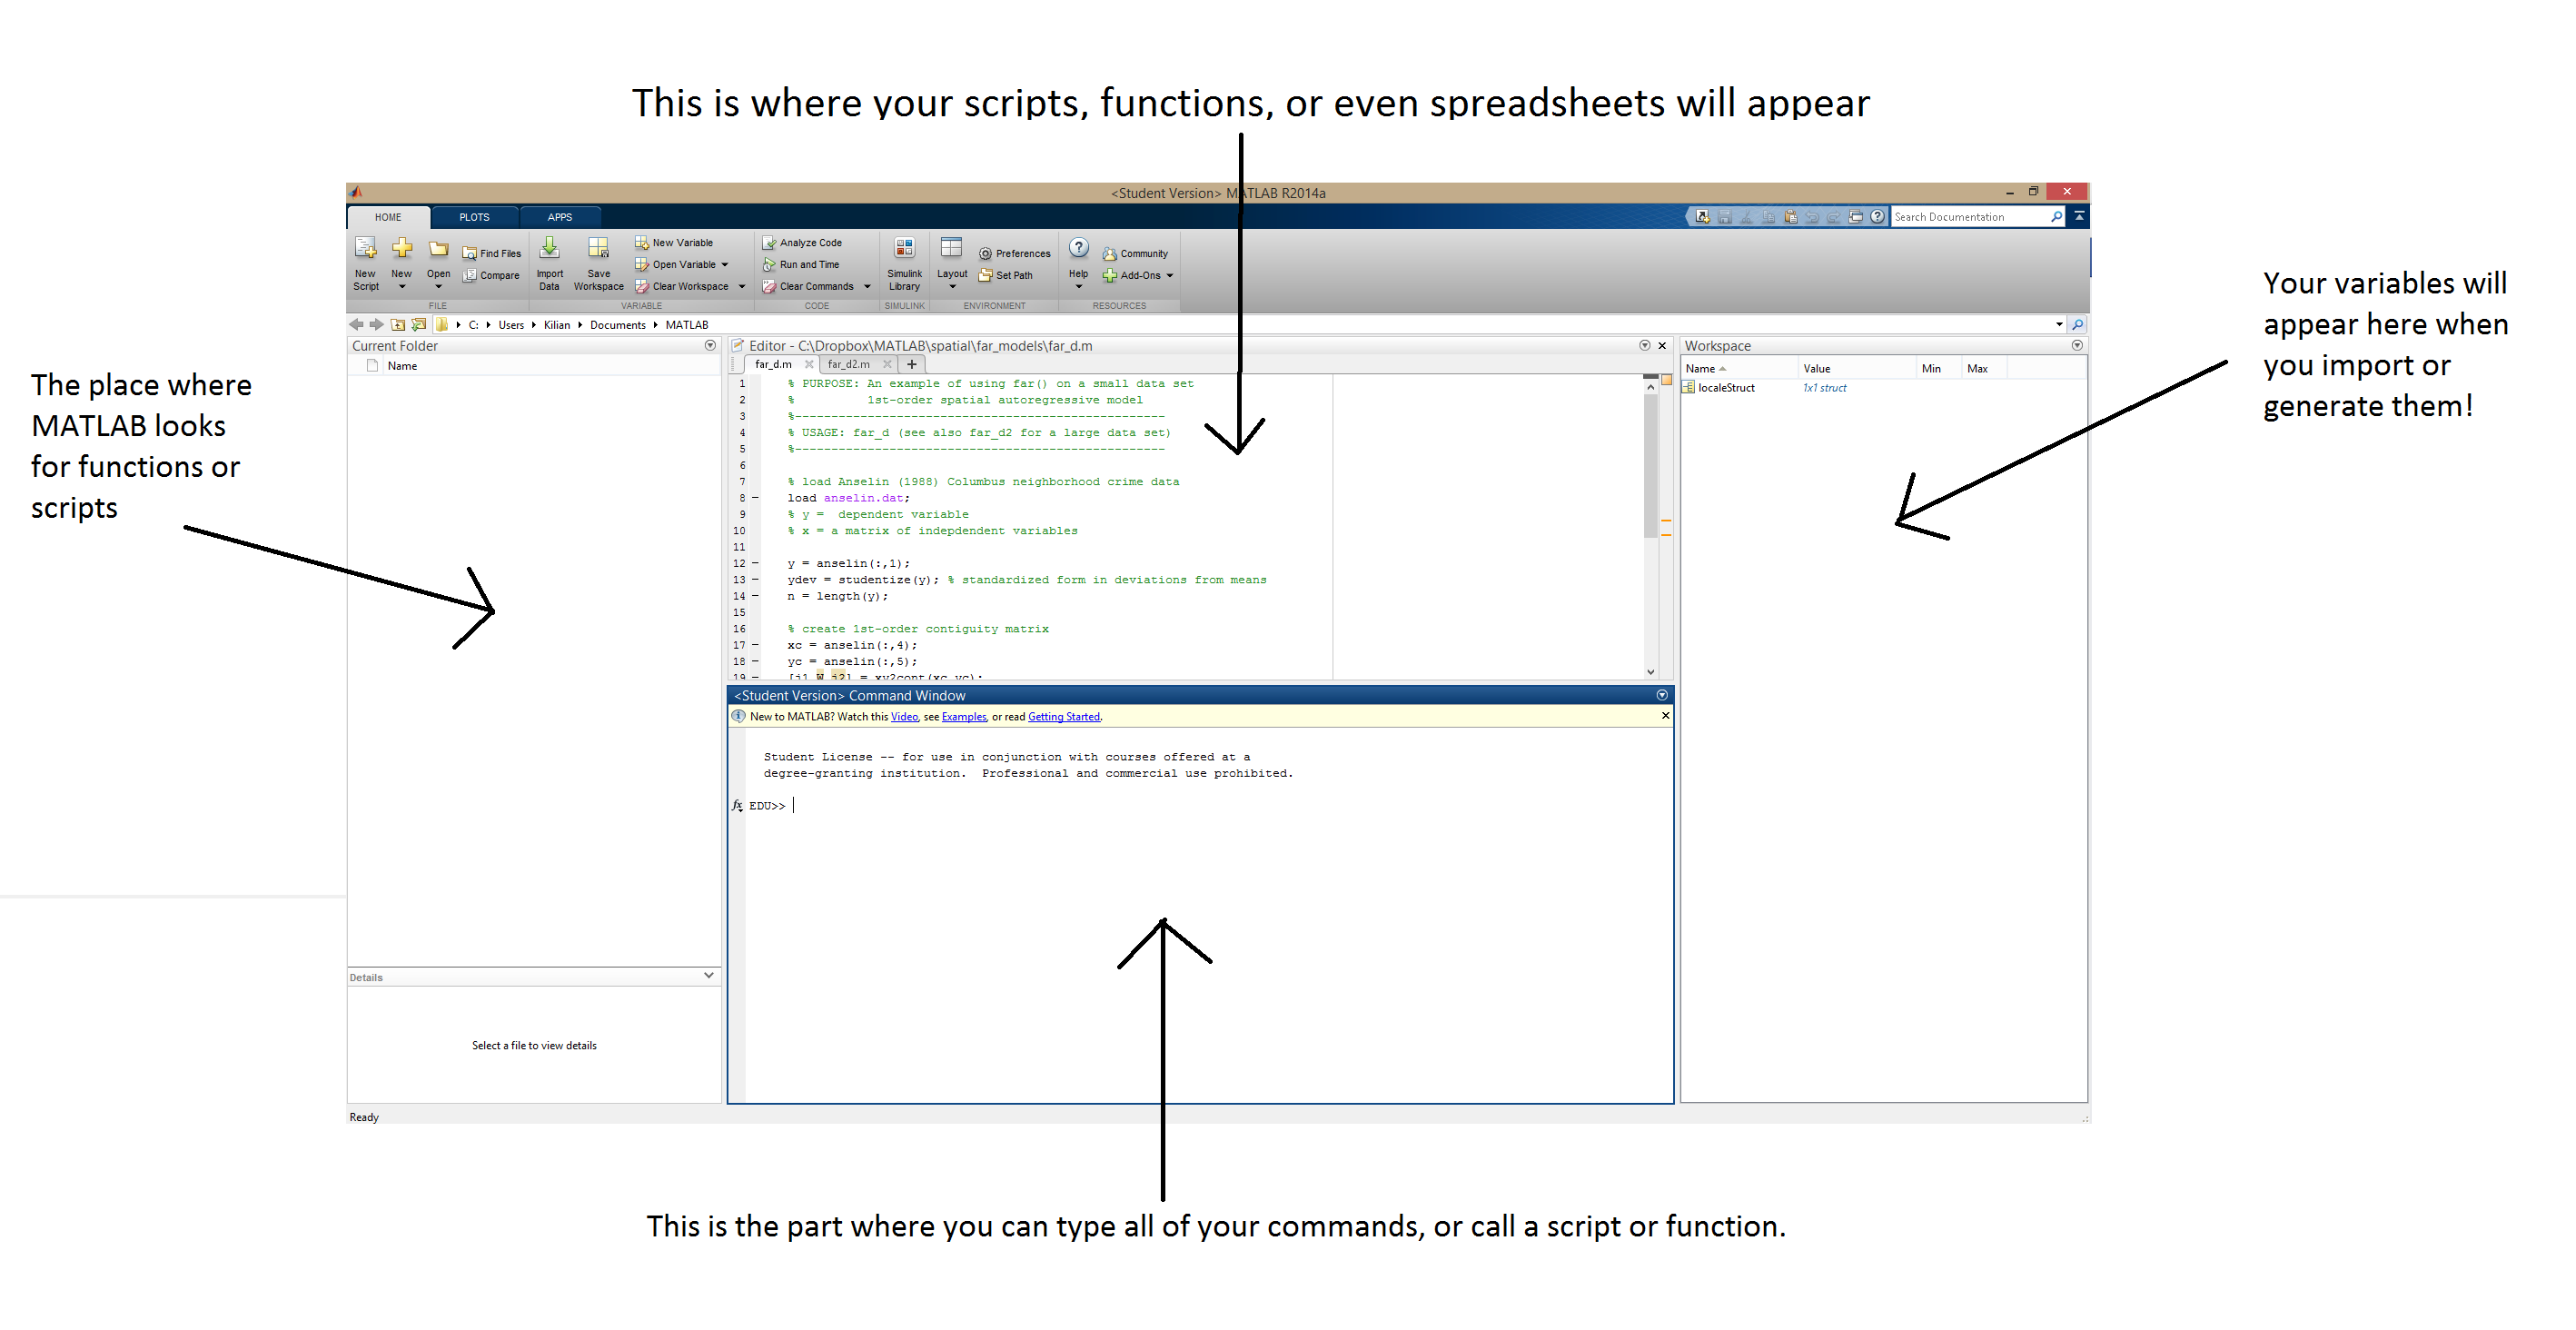
\includegraphics[scale=0.15]{matlabwindows}
\end{center}
\end{figure}
}

\frame{\frametitle{Preliminary MATLAB Commands}
Some things to keep in mind (which will make debugging easier):\\[0.2in]
\begin{itemize}
\item \texttt{addpath}: Adds directory to places MATLAB looks for things.\\[0.1in]
\item \texttt{path}: Displays the current path.\\[0.1in]
\item \texttt{parh2rc}: Adds a path to the places MATLAB searches.\\[0.1in]
\item \texttt{rmpath}: Removes a directory from the search path.\\[0.1in]
\item \texttt{cd}: Changes the current directory.\\[0.1in]
\item \texttt{clc}: Clears the contents of the Command Window.\\[0.1in]
\item \texttt{clf}: Clears the contents of the Figure Window.\\[0.1in]
\end{itemize}
}

\frame{\frametitle{Preliminary MATLAB Commands (Cont.)}
Further useful commands to try and keep in mind:\\[0.2in]
\begin{itemize}
\item \texttt{mkdir newdir}: Like GitBash, mkdir creates a new directory.\\[0.1in]
\item \texttt{Ctrl+C}: Breaks out of loops.\\[0.1in]
\item \texttt{Diary <filename>/Diary on/Diary off}: Creates a log of all your commands, similar to Stata.\\[0.1in]
\item \texttt{who/whos}: Displays a list of variables.\\[0.1in]
\item \texttt{disp(<variablename>)}: Displays the contents of a variable.\\[0.1in]
\item \texttt{docsearch(`phrase')}: Searches the help browser for `phrase'.\\[0.1in]
\item \texttt{helpbrowser}: Opens the help browser\\[0.1in]
\end{itemize}
}

\frame{\frametitle{MATLAB as a Calculator}
Lets open MATLAB and try some commands of our own. The simplest use of MATLAB is as a calculator:\\
\begin{center}
\texttt{EDU>>2+2}
\end{center}
Compare this to:
\begin{center}
\texttt{EDU>>2+2 $\hdots$ \\
+2}
\end{center}
Create an object to hold the result of our calculation:
\begin{center}
\texttt{EDU>>a=2+2;}\\[0.2in]
\end{center}
}

\frame{\frametitle{Some Syntax Notes}
Some things to note here:\\
\begin{itemize}
\item \texttt{>>} is the MATLAB command prompt.\\[0.1in]
\item EDU denotes an educational copy (it may not on UoB terminals).\\[0.1in]
\item +, -, *, / and \^{} have their usual meanings.\\[0.1in]
\item To fit over multiple lines type $\hdots$.\\[0.1in]
\item Note that the use of ; suppresses output.\\[0.1in]
\item You can recall commands with the up and down arrow keys.\\
\end{itemize}
}

\frame{\frametitle{Our First .m File}
To create our first .m file, we have two choices.\\
\begin{enumerate}
\item[1.] Open the MATLAB editor: `New' $\rightarrow$ `Script'.\\
\item[2.] Open up your favorite text editor (e.g. Notepad++).\\
\end{enumerate}
In either, type the same commands from the previous slide:
\begin{center}
\fbox{\begin{minipage}{5em}
\texttt{2+2\\
2+2 ...\\
+2\\
a=2+2}
\end{minipage}}
\end{center}
\begin{itemize}
\item Save/run (`run' in MATLAB', or double click your saved .m file in the file directory). \\
\item Compare results to your commands in the command window.\\
\end{itemize}
} 

\definecolor{mygreen}{RGB}{34,139,34}
\frame{\frametitle{Our Second .m File}
Lets run a slightly more complex .m file to check out more features:\\[0.25in]
\footnotesize
\texttt{
\hspace{19mm}\color{mygreen}\% Example adapted from Frain (2010)\\
\hspace{20mm}\color{black} echo off\\
\hspace{20mm}r=3;\\
\hspace{20mm}volume=(4/3)*pi*r\^{}3;\\
\hspace{20mm}string=['volume of a sphere of radius ' ...\\
\hspace{20mm}num2str(r) ' is ' num2str(volume)];\\
\hspace{20mm}forecast modelyesseasonal\_f\\
\hspace{20mm}disp(string)\\[0.25in]
}
\normalsize
Then you can re-run this to check different values of r.
}

\frame{\frametitle{Our Second .m File (Cont.)}
What features can you spot here that we havent seen before so far?\\[0.1in]
\begin{itemize}
\item \texttt{\color{mygreen}\% Comments are in green and dont affect the code}\\
\item \color{black}\texttt{echo off}
\item \texttt{*}
\item \texttt{string}
\item \texttt{`putting text inside apostrophes'}
\item \texttt{num2str}
\item \texttt{disp}
\item Note the colours if you're using the MATLAB editor.\\[0.2in]
\end{itemize}
Save this in your default working directory as volume\_of\_a\_sphere.m, and then type volume\_of\_a\_sphere into your command window.
}

\frame{\frametitle{A Note on .m Files}
\begin{itemize}
\item In general, note that .m files will regularly adapt the same structure (as on the last slide):\\[0.2in]
\end{itemize}
\begin{enumerate}
\item[1.] Get/Process/Prepare the data.\\[0.1in]
\item[2.] Estimate some form of calculation e.g. $\hat{\beta}=(X'X)^{-1}X'y$ through some MATLAB functions.\\[0.1in]
\item[3.] Report the outputs in terms of graphs and tables.\\[0.1in]
\item[4.] Re-run the estimations changing parameters or specifications to check for robustness.\\[0.1in]
\end{enumerate}
}

\frame{\frametitle{Data input/output}
\begin{itemize}
\item The default data file in MATLAB is a .mat file.\\[0.1in]
\item \texttt{save filename, var1, var2} will save var1 and var2 in `filename.mat'.\\[0.1in]
\item \texttt{load filename, var1, var2} loads `filename.mat'.\\[0.1in]
\item Easiest way to load .csv/xls files - the `Import Data' tool.\\[0.1in]
\item Try it with the data.xls. Try the `Generate Script' function.\\[0.1in] 
\item If you cant find it - run load\_data.m and save it as a .mat: 
\begin{center} 
\texttt{save(`datamat',`IVOLCA', `IVOLCH', `IVOLGB', ... \\`IVOLJP', `IVOLNO', `IVOLSE', `IVOLUS', `IVOLXM')}
\end{center}
\item We could also save a matrix as a csv/xls file e.g. \texttt{M=[ivolca,ivolgb]} and then \texttt{csvwrite(`filename',M)}
\end{itemize}
}

\section{Arrays}\label{two}
\subsection{Vectors, Matrices and Arrays}

\frame{\frametitle{Vectors, Matrices and Arrays}
The basic variable is an Array. Scalars are 1 $\times$ 1, column vectors as n $\times$ 1 and matrices as n $\times$ m. Examples:\\[0.1in]
\begin{itemize}
\item A 1 by 4 matrix (row vector):
\begin{center}
\texttt{x=[1 2 3 4]}
\end{center}
\item A 4 by 1 matrix (column vector):
\begin{center}
\texttt{x=[1;2;3;4]}
\end{center}
\item A 2 by 3 matrix:
\begin{center}
\texttt{x=[1,2,3;4,5,6]}
\end{center}
\item An empty array:
\begin{center}
\texttt{x=[]}
\end{center}
\end{itemize}
}

\frame{\frametitle{A Quick Word on Number Formats}
\begin{itemize}
\item First lets define an arbitrary number:
\begin{center}
\texttt{x=82.828282828282828282}\\[0.1in]
\end{center}
\item Some commands which determine how this is displayed:\\[0.25in]
\end{itemize}
\texttt{
\hspace{18.5mm}format loose \color{mygreen}\%adds in blank lines to space output\\
\hspace{20mm}\color{black}format compact \color{mygreen}\%suppresses blank lines\\
\hspace{20mm}\color{black}format long \color{mygreen}\%displays to 14 decimal places\\
\hspace{20mm}\color{black}format short e \color{mygreen}\%exponential or scientific format\\
\hspace{20mm}\color{black}format long e \color{mygreen}\%long exponential\\
\hspace{20mm}\color{black}format short g \color{mygreen}\%short decimal format\\
\hspace{20mm}\color{black}format bank \color{mygreen}\% currency format of 2 decimals\\
}
}

\frame{\frametitle{A Quick Word on fprintf}
\begin{itemize}
\item The \texttt{fprintf} command prints the results to the command window in a certain way.\\[0.1in]
\item For example, in the following, \% indicates the start of a specification.\\[0.1in]
\item There will be six digits displayed, where 4 are floating point decimals.\\[0.1in]
\item the $\backslash$n indicates the cursor then moves to a new line.\\
\end{itemize}
\begin{center}
\texttt{fprintf (`\%6.2f$\backslash$n',x)}
\end{center}
}

\frame{\frametitle{Basic Matrix Operations}
\begin{itemize}
\item Let's define two matrices and play with them:\\[0.1in]
\begin{center}
\texttt{x = [1,2;3,4]\\
y=[3,7;5,4]}\\[0.1in]
\end{center}
\item Addition:
\begin{center}
\texttt{a=x+y}\\[0.1in]
\end{center}
\item Subtraction:
\begin{center}
\texttt{b=x-y}\\[0.1in]
\end{center}
\item Multiplication:
\begin{center}
\texttt{c=x*y}\\[0.1in]
\end{center}
\item Remember that matrices must `conform'!
\end{itemize}
}

\frame{\frametitle{Matrix Inversion}
\begin{itemize}
\item Lets find the inverse of matrix \texttt{x=[1,2;3,4]}:
\begin{center}
\texttt{a=inv(x)}\\[0.1in]
\end{center}
\item To verify the inverse:
\begin{center}
\texttt{b=x*inv(x)}\\[0.1in]
\end{center}
\item Multiply y by the inverse of x:
\begin{center}
\texttt{c = y*inv(x)}\\
or\\
\texttt{d=y/x}\\[0.1in]
\end{center}
\item Pre-multiply y by the inverse of x:
\begin{center}
\texttt{e=inv(x)*y}\\
or\\
\texttt{f=x$\backslash$y}\\[0.1in]
\end{center}
\end{itemize}
}

\frame{\frametitle{Kronecker Product}
\begin{itemize}
\item Lets now show an example of how to use Kronecker products.\\[0.1in]
\item Define a matrix as before:
\begin{center}
\texttt{x=[1,2;3,4]}\\[0.1in]
\end{center}
\item Then define the always useful identity matrix:
\begin{center}
\texttt{I=eye(2,2)}\\[0.1in]
\end{center}
\item To use this operator:
\begin{center}
\texttt{a=Kron(x,I)}\\[0.1in]
\end{center}
\end{itemize}
}

\frame{\frametitle{Element by Element}
\begin{itemize}
\item As before, define \texttt{x=[1,2;3,4]} and \texttt{y=[5,6;7,8]}.\\[0.1in]
\item To do element by element multiplication:
\begin{center}
\texttt{a=x.*y}
\end{center}
\item For element by element division:
\begin{center}
\texttt{b=y./x}
\end{center}
\item If you try and divide by zero, you will get a warning!\\[0.1in]
\item Define a scalar (e.g. z=2) then try:
\end{itemize}
\begin{center}
\texttt{c=x+z}\\
\texttt{d=x-z}\\
\texttt{e=x*z}\\
\texttt{f=x/z}\\
\texttt{g=x\^{}g}\\
\end{center}
\begin{itemize}
\item \texttt{log}, \texttt{sqrt}, and \texttt{exp} are all element by element.
\end{itemize}
}

\frame{\frametitle{Other Matrix Commands}
\begin{itemize}
\item \texttt{det(x)}, \texttt{rank(x)} and \texttt{trace(x)} work as expected.\\[0.1in]
\item \texttt{diag(x)} where X is a matrix puts diagonal of X in a vector.\\[0.1in]
\item \texttt{diag(x)} where X is a vector outputs a matrix with a diagonal of X and zeros elsewhere.\\[0.1in]
\item \texttt{sum(x)} returns the sum of all elements of a vector, or a row vector of the column sums of a matrix.\\
\item The function \texttt{reshape(A,m,n)} returns the m$\times$n matrix B whose elements are taken column wise from A. This is more complicated, so let's see an example:
\begin{center}
\texttt{x=[1,2,3;4,5,6]\\
reshape(x,3,2)}\\
\end{center}
\end{itemize}
}
\frame{\frametitle{Other Matrix Commands (Cont.)}
The command \texttt{blkdiag(A,B.C)} constructs a block diagonal from matrices. Try:
\begin{center}
\texttt{a=[1,2;3,4]\\
b=[5]\\
c=[6,7;8,9]\\
d=blkdiag(a,b.c)}\\
\end{center}
In order to produce a diagonal matrix D of generalized eigenvalues and a full matrix V whose columns are the corresponding eigenvectors so that A*V = B*V*D:
\begin{center}
\texttt{[V,D]=eig(A)}
\end{center}
}

\frame{\frametitle{Sequences}
\begin{itemize}
\item The colon operator is the easiest way to make a sequence, with the general syntax of
\end{itemize}
\begin{center}
 \texttt{first:increment:last}
\end{center}
\begin{itemize}
\item Try:\\
\end{itemize}
\begin{center}
\texttt{a=[1:3:10]}\\
\end{center}
\begin{itemize}
\item Or to make simple row or column vectors:\\
\end{itemize}
\begin{center}
\texttt{b=[1:4]$'$}\\
\end{center}
\begin{itemize}
\item Note that $'$ creates a transpose of a vector or a matrix.\\
\end{itemize}
}

\frame{\frametitle{Special Matrices}
\begin{itemize}
\item For example, an identity matrix:
\begin{center}
\texttt{a=eye(4)}\\[0.1in]
\end{center}
\item Or a matrix of ones:
\begin{center}
\texttt{b=ones(4,2)}\\[0.1in]
\end{center}
\item Or a matrix of zeros:
\begin{center}
\texttt{c=zeros(3)}\\[0.1in]
\end{center}
\item To return the size of a matrix (rows, columns): \\
\begin{center} \texttt{[nr,nc]=size(x)}
\end{center}
\item We can store random numbers in matrices, vectors or scalars using something like \texttt{d=rand(5)} for random uniform or \texttt{e=randn(5)} for draws from a standard normal distribution.
\end{itemize}
}

\frame{\frametitle{Matrix Manipulation}
\begin{itemize}
\item We can isolate individual elements e.g.: 
\begin{center}
\texttt{x=[1:1:5]\\
y=x(3)}\\[0.1in]
\end{center}
\item Or entire elements using the colon operator e.g.:
\begin{center}
\texttt{x=[1,2;3,4]\\
y=x(2,:)}\\[0.1in]
\end{center}
\item We can also use sub-matrices on the left:
\begin{center}
\texttt{x=[1,2,3,4;5,6,7,8,9;10,11,12,13]\\
x(1:2,[1,4]=[100,99;98,97]}\\[0.1in]
\end{center}
\item We can also make some block assignments:
\begin{center}
\texttt{x(1:2,1:4)=1}\\[0.1in]
\end{center}
\item We can also stack: \texttt{x=[1,2;3,4]} and \texttt{y=[5,6;7,8]}:
\begin{center}
\texttt{z=[x,y]}
\end{center}
\end{itemize}
}

\section{OLS Example}\label{three}
\subsection{An Example Using OLS}
\frame{\frametitle{Regression  Example}
Following Frain (2010), we can now run a simulated OLS:
\begin{equation}
y_t=\beta_1 + \beta_2 x_{2,t} +\beta_3 x_{3,t} +\varepsilon_t
\end{equation}
\begin{itemize}
\item $x_{2,t}$ is a trend variable with values (1,2,...,30).\\[0.1in]
\item $x_{3,t}$ is uniformly distributed on [3,5].\\[0.1in]
\item $\varepsilon_t$ are idd normal random - zero mean, constant variance.\\[0.1in]
\item $\beta_1$=5, $\beta_2=1$, $\beta_3=0.1$.\\[0.1in]
\item $\varepsilon_t$ are iid(0,0.4)\\[0.1in]
\item We will attempt to estimate a large number of regression outputs and compare them with EViews to ensure consistency.\\
\end{itemize}
}

\frame{\frametitle{Regression  Example - Prepare and Process}
\begin{itemize}
\item First lets define the size of our variables:
\begin{center}
\texttt{nsimul=50}\\[0.1in]
\end{center}
\item And our vector of coefficients:
\begin{center}
\texttt{beta=[5,1,0.1]'}\\[0.1in]
\end{center}
\item Then lets generate our three variables:
\begin{center}
\texttt{x1=ones(nsimul,1) \% an array of constants \\
x2=[1:nsimul]' \% a trend \\
x3=rand(nsimul,1)*2+3\% Uniform on [3,5]}\\[0.1in]
\end{center}
\item And finally some other equations:
\begin{center}
\texttt{e=randn(nsimul,1)*0.2\\
X=[x1,x2,x3]\\
y=X*beta+e\\
$[$nobs,nvar$]$=size(X)}
\end{center}
\end{itemize}
}

\frame{\frametitle{Regression  Example - Understanding}
Let's check everyone is up to speed on what's happening:\\[0.2in]
\begin{enumerate}
\item[1.] Why is $x_3$ is defined like this?\\[0.2in]
\item[2.] Why is the residual (e) defined like this?\\[0.2in]
\item[3.] Note how we stacked variables into a matrix.\\[0.2in]
\item[4.] Note that all of our answers will of course be different!\\[0.2in]
%\item[5.] If at any point you are lost - first\_regression.m is on Canvas.\\[0.2in]
\end{enumerate}
}

\frame{\frametitle{Regression  Example - Estimating the Model}
\begin{itemize}
\item Introducing structures:\\[0.3in]
\texttt{
\hspace{18mm}ols.betahat=(X'*X)$\backslash$X'*y\\
\hspace{20mm}ols.yhat=X*ols.betahat\\
\hspace{20mm}ols.resid=y-ols.yhat\\
\hspace{20mm}ols.ssr=ols.resid'*ols.resid\\
\hspace{20mm}ols.sigmasq = ols.ssr/(nobs-nvar)\\
\hspace{20mm}ols.covbeta=ols.sigmasq*inv(X'*X)\\
\hspace{20mm}ols.sdbeta=sqrt(diag(ols.covbeta))\\
\hspace{20mm}ols.tbeta=ols.betahat./ols.sdbeta\\[0.2in]
}
\item Structures can be thought of as branches, or subfolders.\\[0.1in]
\item Useful if you want to try different specifications, or estimators
\end{itemize}
}

\frame{\frametitle{Regression  Example - Evaluating the Model}
\begin{itemize}
\item Lets now evaluate our model using some common metrics\\[0.3in]
\texttt{
\hspace{8mm} ym=y-mean(y)\\
\hspace{10mm} ols.rsqr1=ols.ssr\\
\hspace{10mm} ols.rsqr2=ym'*ym\\
\hspace{10mm} ols.rsqr=1.0-ols.rsqr1/ols.rsqr2\\
\hspace{10mm} ols.rsrq1=ols.rsqr1/(nobs-nvar)\\
\hspace{10mm} ols.rsqr2=ols.rsqr2/(nobs-1)\\
\hspace{10mm} ols.rbar=1-(ols.rsqr1/ols.rsqr2)\\
\hspace{10mm} ols.ediff=ols.resid(2:nobs)-ols.resid(1:nobs-1)\\
\hspace{10mm} ols.dw=(ols.ediff'*ols.ediff)/ols.ssr}\\[0.2in]
\item Now we have estimated everything we will need to proceed.
\end{itemize}

}



\frame{\frametitle{Regression  Example - Evaluation Outputs}
\begin{itemize}
\item Lets now get MATLAB to present the results to us.\\[0.1in]
\item First, lets focus on the evaluation outputs using fprintf:\\[0.25in]
\texttt{
\hspace{8mm} fprintf(`R-squared = \%9.4f $\backslash$n', ols.rsqr);\\
\hspace{10mm} fprintf(`Rbar-squared = \%9.4f $\backslash$n `, ols.rbar);\\
\hspace{10mm} fprintf(`sigma\^{}2=\%9.4f $\backslash$n `,ols.sigmasq);\\
\hspace{10mm} fprintf(`S.E.=\%9.4f $\backslash$n `,sqrt(ols.sigmasq));\\
\hspace{10mm} fprintf(`Durbin-Watson = \%9.4f $\backslash$n ` ,ols.dw);\\
\hspace{10mm} fprintf(`Nobs, Nvars =\%6d, \%6d $\backslash$n ` ,nobs,nvar);\\[0.2in]
}
\item To get a rudimentary estimation output, type something like:
\begin{center}
\texttt{coeffs=[ols.betahat ols.sdbeta ols.tbeta]}
\end{center}
\end{itemize}
}


\frame{\frametitle{Regression  Example - Coefficient Output}
\begin{itemize}
\item Now lets produce the formatted output::\\[0.25in]
\footnotesize
\begin{center}
\texttt{fprintf(`\%12s \%12s \%12s \%12s \%12s $\backslash$n', ... \\
'Variable','Coefficient','Standard Error','t-statistic')\\[0.15in]
fprintf(`\%12s \%12.6f \%12.6f \%12.6f $\backslash$n',`Const', ...\\
ols.betahat(1), ols.sdbeta(1), ols.tbeta(1))\\[0.15in]
fprintf(`\%12s \%12.6f \%12.6f \%12.6f $\backslash$n', `Trend',...\\
ols.betahat(2), ols.sdbeta(2), ols.tbeta(2))\\[0.15in]
fprintf(`\%12s \%12.6f \%12.6f \%12.6f $\backslash$n', `Var2',...\\
ols.betahat(3), ols.sdbeta(3), ols.tbeta(3))\\[0.1in]
}
\end{center}
\normalsize
\item A fairly standard regression output as per other softwares.\\[0.1in]
\item Note the results change every time we run the .m file (why?).\\[0.1in]
\end{itemize}
}


\frame{\frametitle{Introducing Plots}
\begin{itemize}
\item This might be a nice time to introduce plots:\\[0.1in]
\begin{center}
\texttt{
plot(x2,ols.resid)\\
title(`Graph Title')\\
xlabel(`Time')\\
ylabel(`Residual')\\
}
\begin{figure}
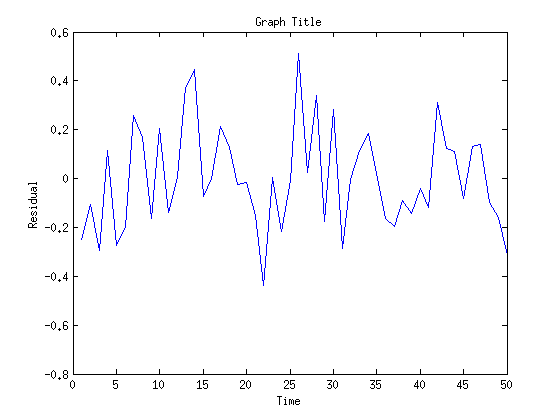
\includegraphics[scale=0.35]{residuals}
\end{figure}
\end{center}
\end{itemize}
}

\frame{\frametitle{Regression Example - Output}
\begin{itemize}
\item Your command window should now look something like this:
\begin{figure}
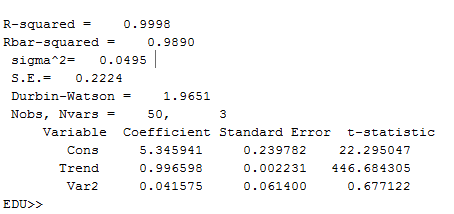
\includegraphics[scale=0.6]{first_regression_results}
\end{figure}
\item (Your results will be different as we're using simulated data!)
\end{itemize}
}
\frame{\frametitle{Regression  Example - Checking Results}
\begin{itemize}
\item Copy your variables x1, x2 and x3 along with your dependent - y into EViews (undated, 50 obs).\\[0.2in]
\item Then run: \texttt{equation eqcheck.ls y1 x1 x2 x3}\\[0.2in]

\begin{figure}
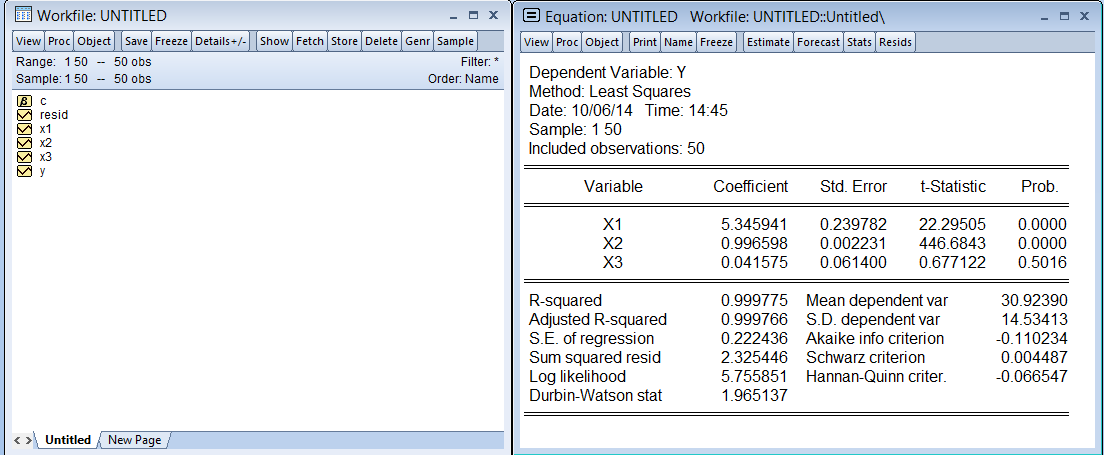
\includegraphics[scale=0.3]{eviewsoutput}
\end{figure}

\end{itemize}
}

\section{Control Statements}\label{four}
\subsection{Decision and Loop Structures.}
\frame{\frametitle{Decision and Loop Structures}
\begin{itemize}
%\item Four main control structures in MATLAB. The first is an \textbf{IF}:
\item \textbf{if statements} take the general form of:\\[.1in]
\texttt{
\hspace{29mm}\color{blue}if \color{black} condition\\
\hspace{35mm}statement\\
\hspace{30mm}\color{blue}end}\\[.1in]
\item Conditions can include the following operators: \\[.1in]
\begin{center}
\texttt{$==, \sim =, <, >, >=, <=, \&, \& \&, |, ||, xor, all, any$}\\[.1in]
\end{center}
\item We can then extend this to \texttt{else} and \texttt{elseif}:\\[.1in]
\texttt{
\small
\hspace{29mm} \color{blue}if \color{black} conditions1\\
\hspace{35mm} statements1\\
\hspace{30mm} \color{blue}elseif \color{black} conditions2\\
\hspace{35mm} statements2\\
\hspace{30mm} \color{blue}else\color{black}\\
\hspace{35mm} statements3\\
\hspace{30mm} \color{blue} end\color{black}}\\
\normalsize
\end{itemize}
}

\frame{\frametitle{Decision and Loop Structures (Cont.)}
\begin{itemize}
\item The next `flow of control' structure we will consider is a \textbf{for} loop:\\[.1in]
\end{itemize}
\texttt{
\hspace{29mm}\color{blue} for \color{black} variable = expression\\
\hspace{35mm}statements\\
\hspace{30mm}\color{blue}end\\}
\begin{itemize}
\item To see how it works, consider the following example:\\[.1in]
\end{itemize}
\texttt{
\hspace{29mm}Balance = 1000; \color{mygreen}\%initialize Balance \\
\hspace{30mm}\color{blue}for \color{black} year = 1:30 \\
\hspace{35mm}BalanceVec(year) = (1.08)*Balance; \\
\hspace{35mm}Balance = BalanceVec(year); \\
\hspace{30mm}\color{blue}end \\
\color{black}\hspace{30mm}plot(1:30, BalanceVec) \\
}
}



\frame{\frametitle{Decision and Loop Structures (Cont.)}
\begin{itemize}
\item The general format of a \textbf{while} statement is similar:\\[.1in]
\end{itemize}
\texttt{
\hspace{28mm}\color{blue}while \color{black} conditions\\
\hspace{35mm}statements\\
\hspace{30mm}\color{blue}end\color{black}\\[.2in]
}
\begin{itemize}
\item Lets see an example below:\\[.2in]
\end{itemize}
\texttt{
\hspace{28mm}balance = 50;\\
\hspace{30mm}year = 0\\
\hspace{30mm}\color{blue}while \color{black} balance <100\\
\hspace{35mm}balance = (1.09)*balance\\
\hspace{35mm}year=year+1\\
\hspace{30mm}\color{blue}end\\
\hspace{30mm}year\color{black}, balance\\
}
}

%\frame{\frametitle{Decision and Loop Structures (Cont.)}
%\begin{itemize}
%\item Finally, lets consider switches:\\
%\begin{center}
%\texttt{
%mynumber = input('Enter a number:');\\
%switch mynumber\\
%    case -1\\
%        disp('negative one');\\
%    case 0\\
%        disp('zero');\\
%    case 1\\
%        disp('positive one');\\
%    otherwise\\
%        disp('other value');\\
%end\\}
%\end{center}
%\end{itemize}
%}
%


\section{Functions}\label{five}
\subsection{User Defined Functions.}
\frame{\frametitle{User Defined Functions}
\begin{itemize}
\item MATLAB gvies you the ability to write your own functions.\\[0.1in]
\item They can then be used just like native functions.\\[0.1in]
\item Up until now, we've used what are called `script' files.\\[0.1in]
\item Note:  The namze of the file should match the name of the first function in the file.\\[0.1in]
\item From MathWorks:\\
\begin{center}
\textit{
\color{blue}function\color{black} [y1,...,yN] = myfun(x1,...,xM) declares a function named myfun that accepts inputs x1,...,xM and returns outputs y1,...,yN.}\\[0.1in]
\end{center}
\item Note that the outputs are in [ ], and inputs are in ( ).\\

\end{itemize}
}



\frame{\frametitle{General Function Structure}
Generally, a function looks something like this.
\begin{figure}
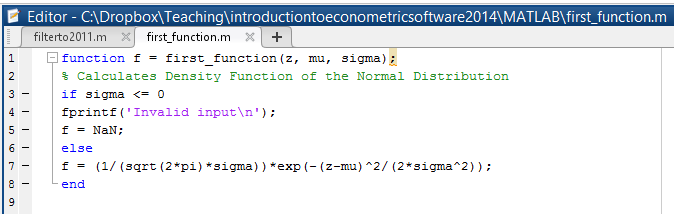
\includegraphics[scale=0.60]{functionshot}
\end{figure}
}


\frame{\frametitle{Our First User Defined Function}
\begin{itemize}
\item Now we'll write a function which estimates the density function of a normal distribution. Recall:\\[0.1in]
\begin{equation}
\frac{1}{\sqrt{2 \pi \sigma}} exp -\frac{(x-\mu)^2}{2\sigma^2}
\end{equation}\\[0.1in]
\item Note that the three inputs to our function are going to be $x$, $\mu$, and $\sigma$.\\[0.1in]
\item After evaluating it for specific values, we are going to plot over an interval.\\
\end{itemize}
}


\frame{\frametitle{A Function for the Density of  Normal Distribution}

\begin{itemize}
\item Just as with scripts, click `New $\rightarrow$ Function' or save as first\_function.m (also on Canvas).\\[0.2in]
\end{itemize}
\small
\texttt{
\hspace{19mm}\color{blue}function \color{black}  f = first\_function(z, mu, sigma);\\
\hspace{20mm}\color{mygreen}\% Calculates Density Function of the Normal Distribution\\
\hspace{20mm}\color{blue}if \color{black} sigma $<$= 0\\
\hspace{25mm}\color{black}fprintf(`Invalid input$\backslash$n');\\
\hspace{20mm}\color{blue}if sigma\color{black} = NaN;\\
\hspace{20mm}\color{blue}else \\
\hspace{25mm}\color{black}f = (1/(sqrt(2*pi)*sigma))*exp(-(z-mu)\^{}2/(2*sigma\^{}2));\\
\hspace{20mm}\color{blue}end\\
}
}
\normalsize

\frame{\frametitle{Density of  Normal Distribution (Cont.)}
\begin{itemize}
\item We can then get help on this function from typing: \\
\begin{center}
\texttt{help first\_function}\\[0.2in]
\end{center}
\item We can evaluate our function at a point (.e.g zero):\\
\begin{center}
\texttt{first\_function(0,0,1)}\\[0.2in]
\end{center}
\item And finally, we can plot our function on the interval [-5,5]:\\
\begin{center}
\texttt{fplot(`normaldensity(x,0,1)', [-5,5])}

\begin{figure}
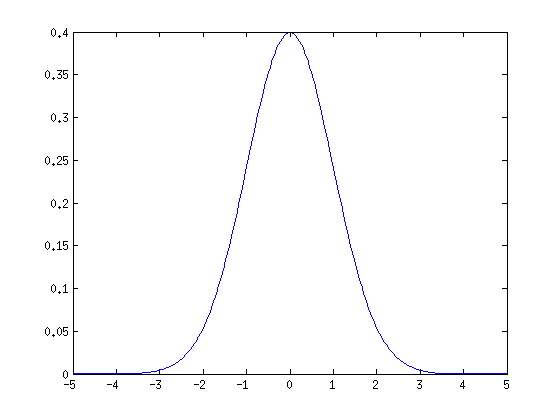
\includegraphics[scale=0.25]{normaldistribution}
\end{figure}
\end{center}
\end{itemize}
}





\section{Toolboxes}\label{six}
\subsection{Applications of the LeSage Toolbox}
\frame{\frametitle{LeSage Toolbox}
\begin{itemize}
\item A `toolbox' is a related set of MATLAB functions aimed at solving a particular class of problems.\\[0.1in]
\item Toolboxes of functions useful in signal processing, optimization, statistics, finance/a host of other areas available from
 MathWorks.\\[0.1in]
\item Most popular for econometrics is written by James LeSage:
\begin{center}
\url{www.spatial-econometrics.com}\\[0.1in]
\end{center}
\item It is split (handily) into libraries: Regression, Utility Functions, Diagnostics, VAR/VECMs, MCMCMs, Limited Dependents, SEMs, Distributions, Optimizations, etc. \\[0.1in]
\item Of particular interest is the \emph{Spatial Econometrics} Library.\\[0.1in]
\end{itemize}
}

\frame{\frametitle{Installing Toolboxes or Functions}
\begin{itemize}
\item To install the toolbox, a specific library, or a function:\\[0.1in]
\end{itemize}
\begin{enumerate}
\item[1.] Download the toolbox.
\item[2.] If it's zipped, extract it: at home, somewhere like:\\[0.1in]
\begin{center}
\texttt{C:$\backslash$Program Files$\backslash$MATLAB$\backslash$R2014a$\backslash$toolbox}
\end{center}
\item[3.] Add a new folder, call it `econ'.\\[0.1in]
\item[4.] Or on the University computers, you will have to extract to somewhere like `econ' in your documents.\\[0.1in]
\item[5.] Just as before, you will have to navigate to it in the MATLAB window `current folder' window, right click, and:\\
\begin{center}
\texttt{Add to path $\rightarrow$ Selected Folders and Subfolders}
\end{center}
\end{enumerate}
}


\frame{\frametitle{LeSage Toolbox}
If everything has gone right, you should have a list of the librarys within the Toolbox added to the Current Folder:
\begin{figure}
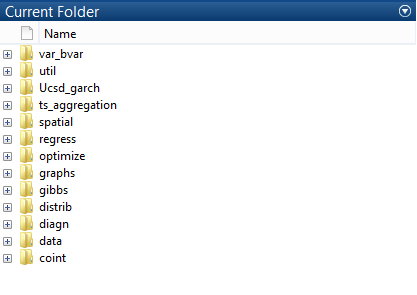
\includegraphics[scale=0.65]{lesagetoolbox}
\end{figure}
}

\frame{\frametitle{REGRESS}
\begin{itemize}
\item The first thing which we are going to do is use the REGRESS library .\\[0.2in]
\item Then, we'll compare our results with `first\_regression' which we wrote earlier.\\[0.2in]
\item After running this file, we will use the y and X objects.\\[0.2in]
\item After running this file, be sure to delete or rename the `ols' structure, or MATLAB will get confused, giving you error:
\begin{center}
\small\texttt{Subscript indices must either be real positive integers or logicals.}\normalsize\\[.2in]
\end{center}
\item This is because our regression \emph{function} in the LeSage Toolbox is called `ols' also.
\end{itemize}
}

\frame{\frametitle{Checking OLS and first\_regression}
\begin{itemize}
\item To use the LeSage function: \texttt{results=ols(y,X)}.
\end{itemize}
\begin{figure}
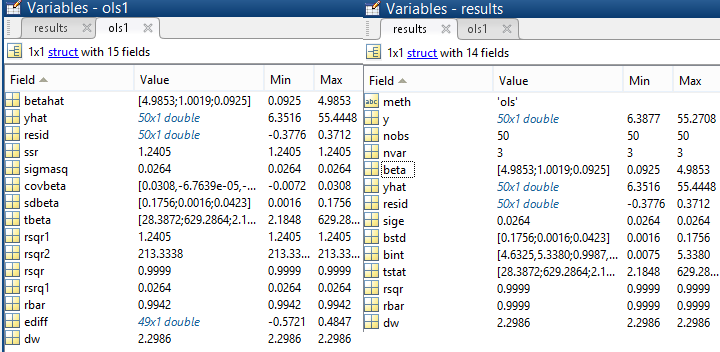
\includegraphics[scale=0.4]{compare}
\end{figure}
\begin{itemize}
\item Remember we are generating random variables each time.\\[0.1in]
\item Name our structure anything (e.g. \texttt{olsresults=ols(y,X)}).\\[0.1in]
\end{itemize}
}

%\frame{\frametitle{Graphs Library - TSPlot}
%\begin{itemize}
%\item Lets try a couple of examples from the Graphs library:
%\end{itemize}
%\begin{center}
%\texttt{cstr = cal(2000,1,12);\\
%tsplot(x3,cstr,'Variable Three')}
%\end{center}
%\begin{figure}
%\caption{An Example of TSPLOT}
%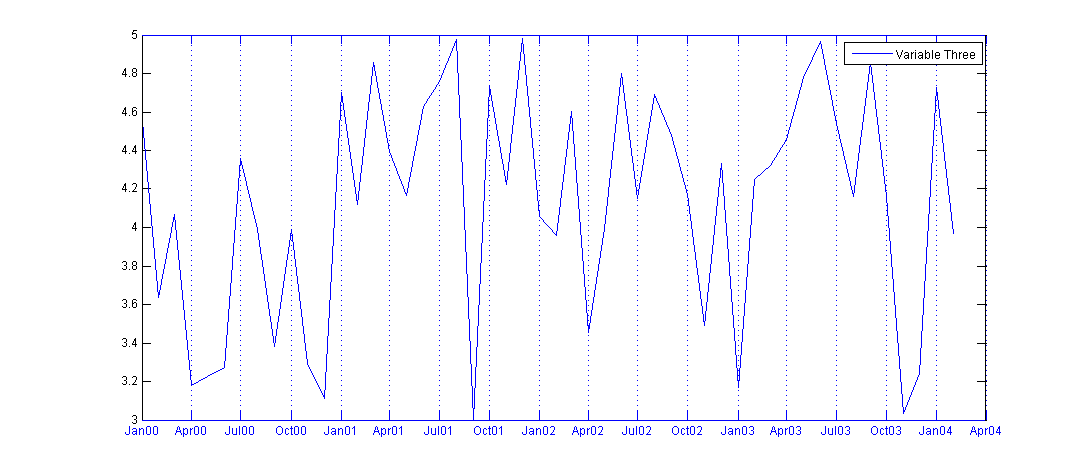
\includegraphics[scale=0.2]{tsplot.png}
%\end{figure}
%}
%
%\frame{\frametitle{Graphs Library - Plot Density}
%\begin{itemize}
%\item As a second and final example of plotting from the Graphs library, use:
%\end{itemize}
%\begin{center}
%\texttt{pltdens(x3)}
%\end{center}
%\begin{figure}
%\caption{An Example of PLTDENS}
%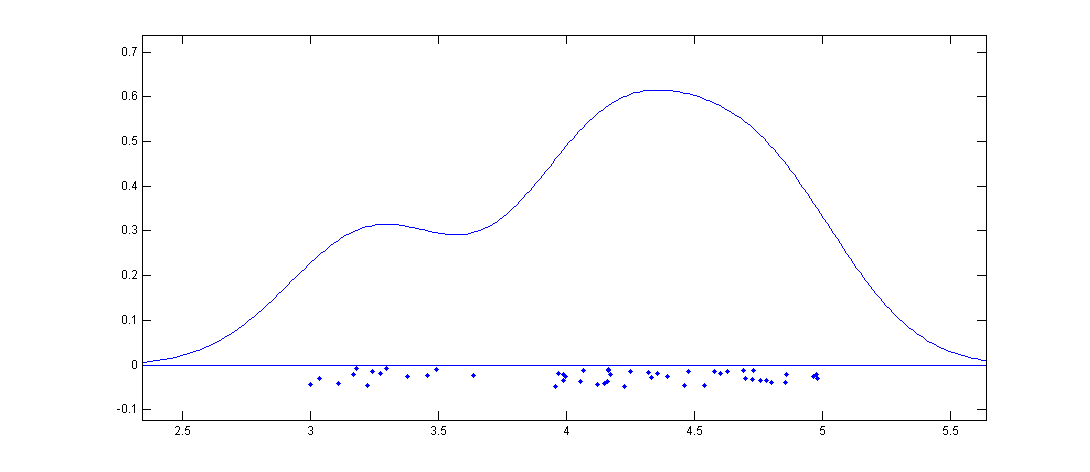
\includegraphics[scale=0.2]{pltdens.png}
%\end{figure}
%}
%
%\frame{\frametitle{VAR\_BVAR Library}
%\begin{itemize}
%\item In the var\_bvar library, lets generate an AR(4) model:
%\end{itemize}
%\begin{center}
%\texttt{info.const=0 \%: No constant\\
%results=ar(y,4,info)}
%\begin{figure}
%\caption{An Example of an AR(4) Model}
%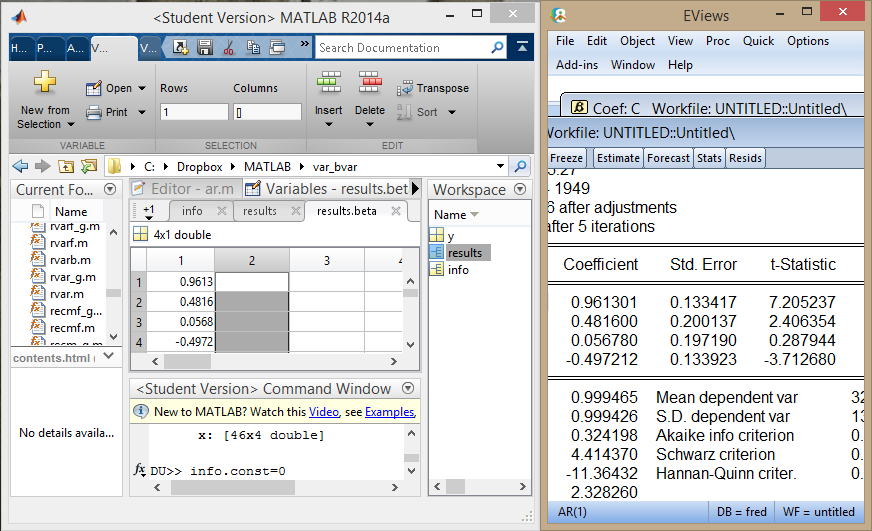
\includegraphics[scale=0.25]{ar4results.png}
%\end{figure}
%\end{center}
%}
%
%
%\frame{\frametitle{VAR\_BVAR Library (Cont.)}
%\begin{itemize}
%\item Now lets try a VAR(4) model:
%\end{itemize}
%\begin{center}
%\texttt{Z=[y,x3]\\
%varresults=vare(Z,4)}
%\begin{figure}
%\caption{An Example of a VAR(4) Model}
%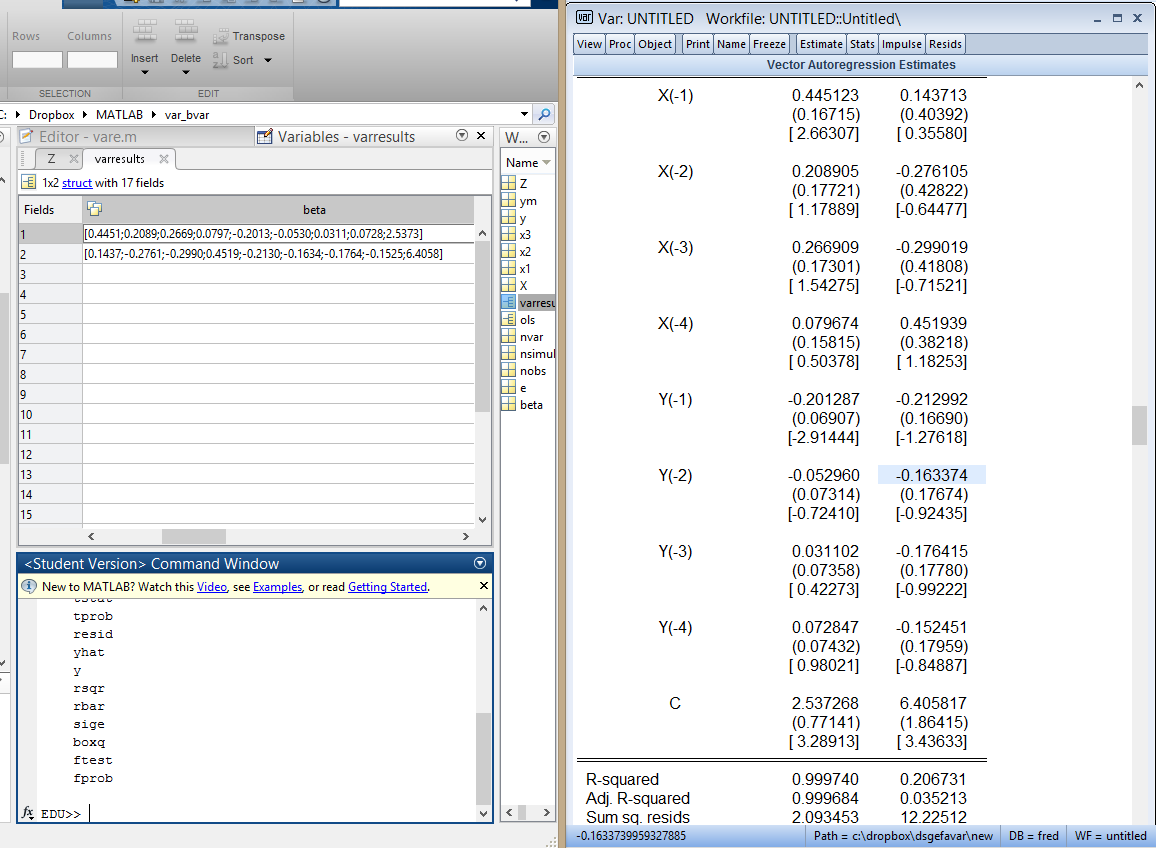
\includegraphics[scale=0.2]{var4results.png}
%\end{figure}
%\end{center}
%}
%
%
%\frame{\frametitle{VAR\_BVAR Library (Cont.)}
%\begin{itemize}
%\item Now lets try forecasting from this VAR(4) model.\\[0.1in]
%\item Forecast endogenous vector of variables Z, with 4 lags, 1 period ahead, starting from the 51st (1 period out of sample) forecast.\\[0.1in]
%\end{itemize}
%\begin{center}
%\texttt{ylevf=varf(Z,4,1,51)}
%\begin{figure}
%\caption{An Example of Forecasting from a VAR(4) Model}
%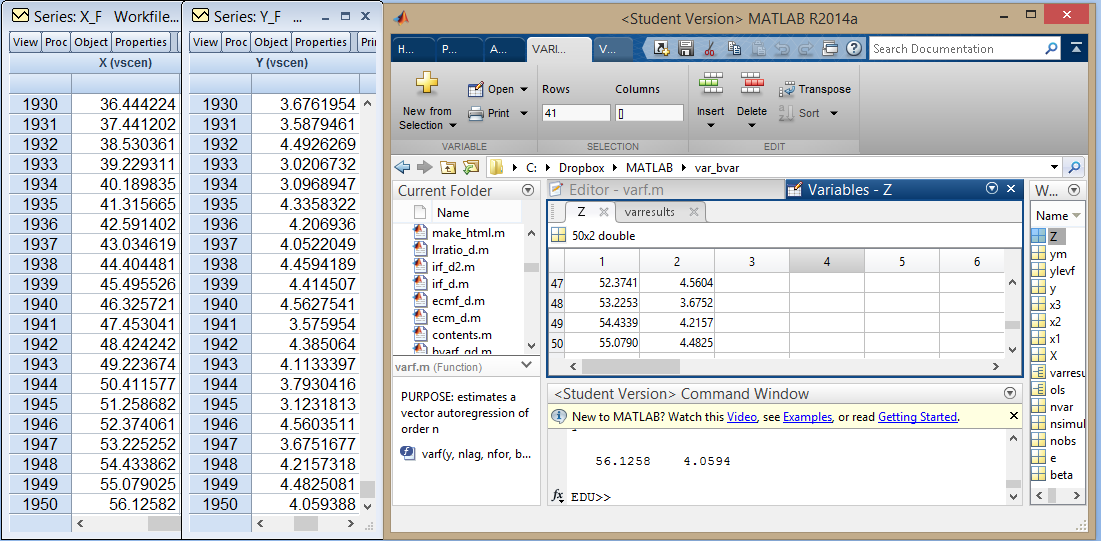
\includegraphics[scale=0.2]{var4forecast.png}
%\end{figure}
%\end{center}
%}
%
%\frame{\frametitle{Coint Library}
%\begin{itemize}
%%\item In `Coint', we can find a discrepancy with the ADF tests.\\[0.1in]
%\item Estimate an ADF test with 4 lags, a constant and time trend:\\
%\end{itemize}
%\begin{center}
%\texttt{adfresults=adf(y,1,4)}
%\begin{figure}
%\caption{An Example of How Results Can Sometimes Differ}
%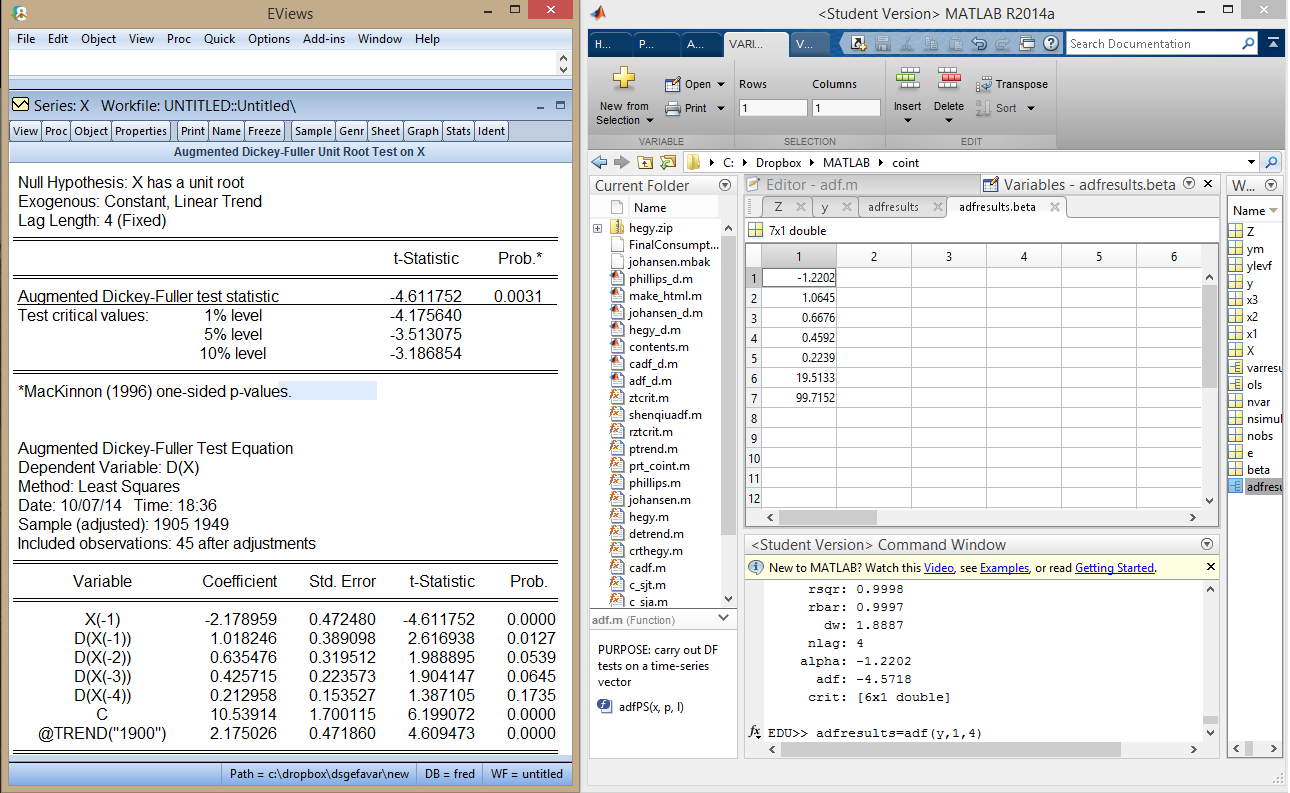
\includegraphics[scale=0.15]{adfresults.png}
%\end{figure}
%\end{center}
%\begin{itemize}
%\item Results are slightly different (can anyone guess why?)
%\end{itemize}
%}

\frame{\frametitle{Application: Spatial Econometrics}
\begin{itemize}
\item We may turn to the LeSage toolbox for spatial econometrics.\\[0.1in]
\item Spatial econometrics is necessary because of spatial dependence or spatial heterogeneity.\\[0.1in]
\item First of all, we must quantify some locational aspects of our data (i.e. address).\\[0.1in]
\item From this, we obtain their latitude and longtitude. \\[0.1in]
\item We can calculate some kind of weighting matrix.\\[0.1in]
\item `Spatial' routines need other functions (`Utilities').\\[0.1in]
\item See the following guide to the Spatial Library:
\small
\begin{center}
\color{blue}\url{http://www.spatial-econometrics.com/html/wbook.pdf}
\end{center}
\normalsize
\end{itemize}
}

\frame{\frametitle{Application: Spatial Econometrics (Cont.)}
\begin{itemize}
\item The most simple example to consider is the FAR model:
\begin{equation}
y=\rho W y + \varepsilon
\end{equation}
\begin{equation}
 \varepsilon \sim N(0,\sigma^2 I_n)
\end{equation}
\item The least squares estimator would yield:
\begin{equation}
\hat{\rho}=(y'W'Wy)^{-1}y'W'y
\end{equation}
\item However, lets show that this estimator is unbiased:
\begin{equation}
E(\hat{\rho})=(y'W'Wy)^{-1}y'W'(\rho Wy+\varepsilon)
\end{equation}
\begin{equation}
E(\hat{\rho})=\rho+(y'W'Wy)^{-1}y'W'\varepsilon
\end{equation}
\item Anselin (1988) also establishes inconsistency.
\end{itemize}
}

\frame{\frametitle{Application: Spatial Econometrics (Cont.)}
\begin{itemize}
\item Find the \textbf{far} and \textbf{far\_d} function/script in the Spatial Library.\\[0.1in]
\item This uses the dataset of Anselin (1988): Columbus neighborhood crime data.\\[0.1in]
\item The functions use maximum likelihood estimators and sparse matrices.\\[0.1in]
\item Sparse matrices are necessary otherwise inverting the large matrices would be extremely difficult.\\[0.1in]
\item Many W matrices in the literature have many zero elements (e.g. `nearest neighbor' or contiguity).\\[0.1in]
\item If a problem has $<500$ obs, it computes the theoretical information matrix, if $>500$,  computes a numerical Hessian.\\[0.1in]
\end{itemize}
}



\frame{\frametitle{Application: Spatial Econometrics (Cont.)}
\begin{itemize}
\item Call the example FAR script \texttt{far\_d}. Hopefully your results are similar to:
\end{itemize}
\begin{figure}
\caption{Output Results for far\_d}
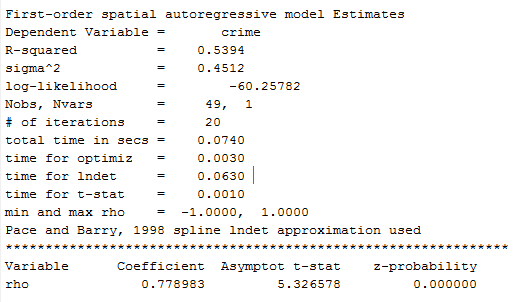
\includegraphics[scale=0.4]{far_d.png}
\end{figure}
}

\frame{\frametitle{Application: Spatial Econometrics (Cont.)}
\begin{itemize}
\item In addition to this, you can also plot the spatial weighting matrix using the command:
\end{itemize}
\begin{center}
\texttt{spy(D)}
\end{center}
\begin{figure}
\caption{Spatial Weighting Matrix for far\_d}
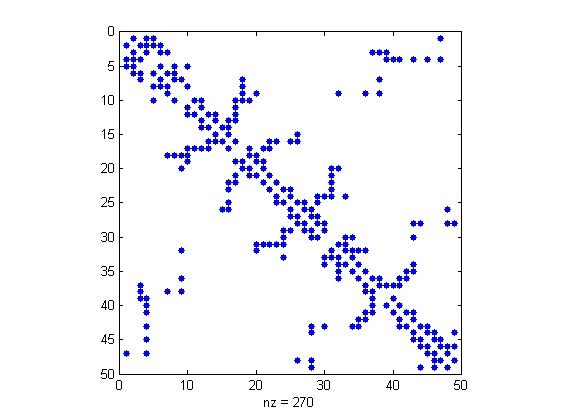
\includegraphics[scale=0.35]{spy(w).png}
\end{figure}
}

\section{Homework}\label{seven}
\subsection{Optional Homework}
\frame{\frametitle{Optional Homework Assignment}
\begin{itemize}
\item Taken from Pouliot and Lampis (2014):\\[0.25in]
\fbox{\begin{minipage}{30em}
Write a function called \color{red}mydiag\color{black}{} that returns a diagonal matrix if the input is a vector and returns the diagonal entries of the matrix if the input is a matrix. Use the \texttt{max}, \texttt{min} and \texttt{size}.
\end{minipage}}
\end{itemize}
}
\end{document}